\chapter{Resultat}

Nedan presenteras det system som utvecklats.

\section{Installation av systemet}
Ett av kraven från kunden var att kunna installera systemet på sin egna server
och låta det köra därifrån. För att underlätta för kunden vid installationen
skapades en installationsfil som laddar ner systemets filer, fixar
inställningar för databasen och även ställer frågor om vilka
tredjepartstjänster som ska användas. Installationsfilen anpassar sedan
systemet utefter de svar som fås av användaren vid installation. Stegen för
installationen kan ses i figur \ref{fig:installation}.

\begin{figure}[!h]
\centering
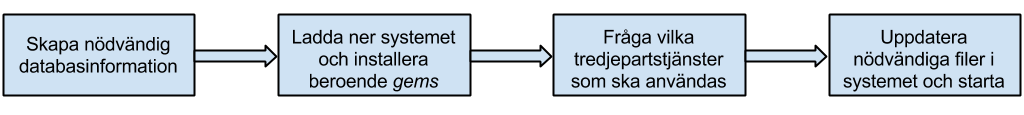
\includegraphics[width=0.8\textwidth]{figures/installation.png}
\caption{De steg som installationsfilen tar för att installera systemet.}
\label{fig:installation}
\end{figure}

\section{Programdesign}

Systemet är uppdelat i två huvudsakliga delar: server och klient.
Javascriptklienten skickar och tar emot data från servern, som presenterar
resultatet i JSON (\emph{Javascript object notation}).

\subsection{Ruby on Rails}

Följande \emph{models} valdes att användas för systemet. Relationerna mellan
dem är specificerade i figur \ref{fig:models}. Modellen \texttt{BruseFile} fick
det namnet eftersom \texttt{File} är ett reserverat ord i Ruby.

\begin{Figure}
  % center it!
  \centering
    % adjust width as you like, include image from optional folder
    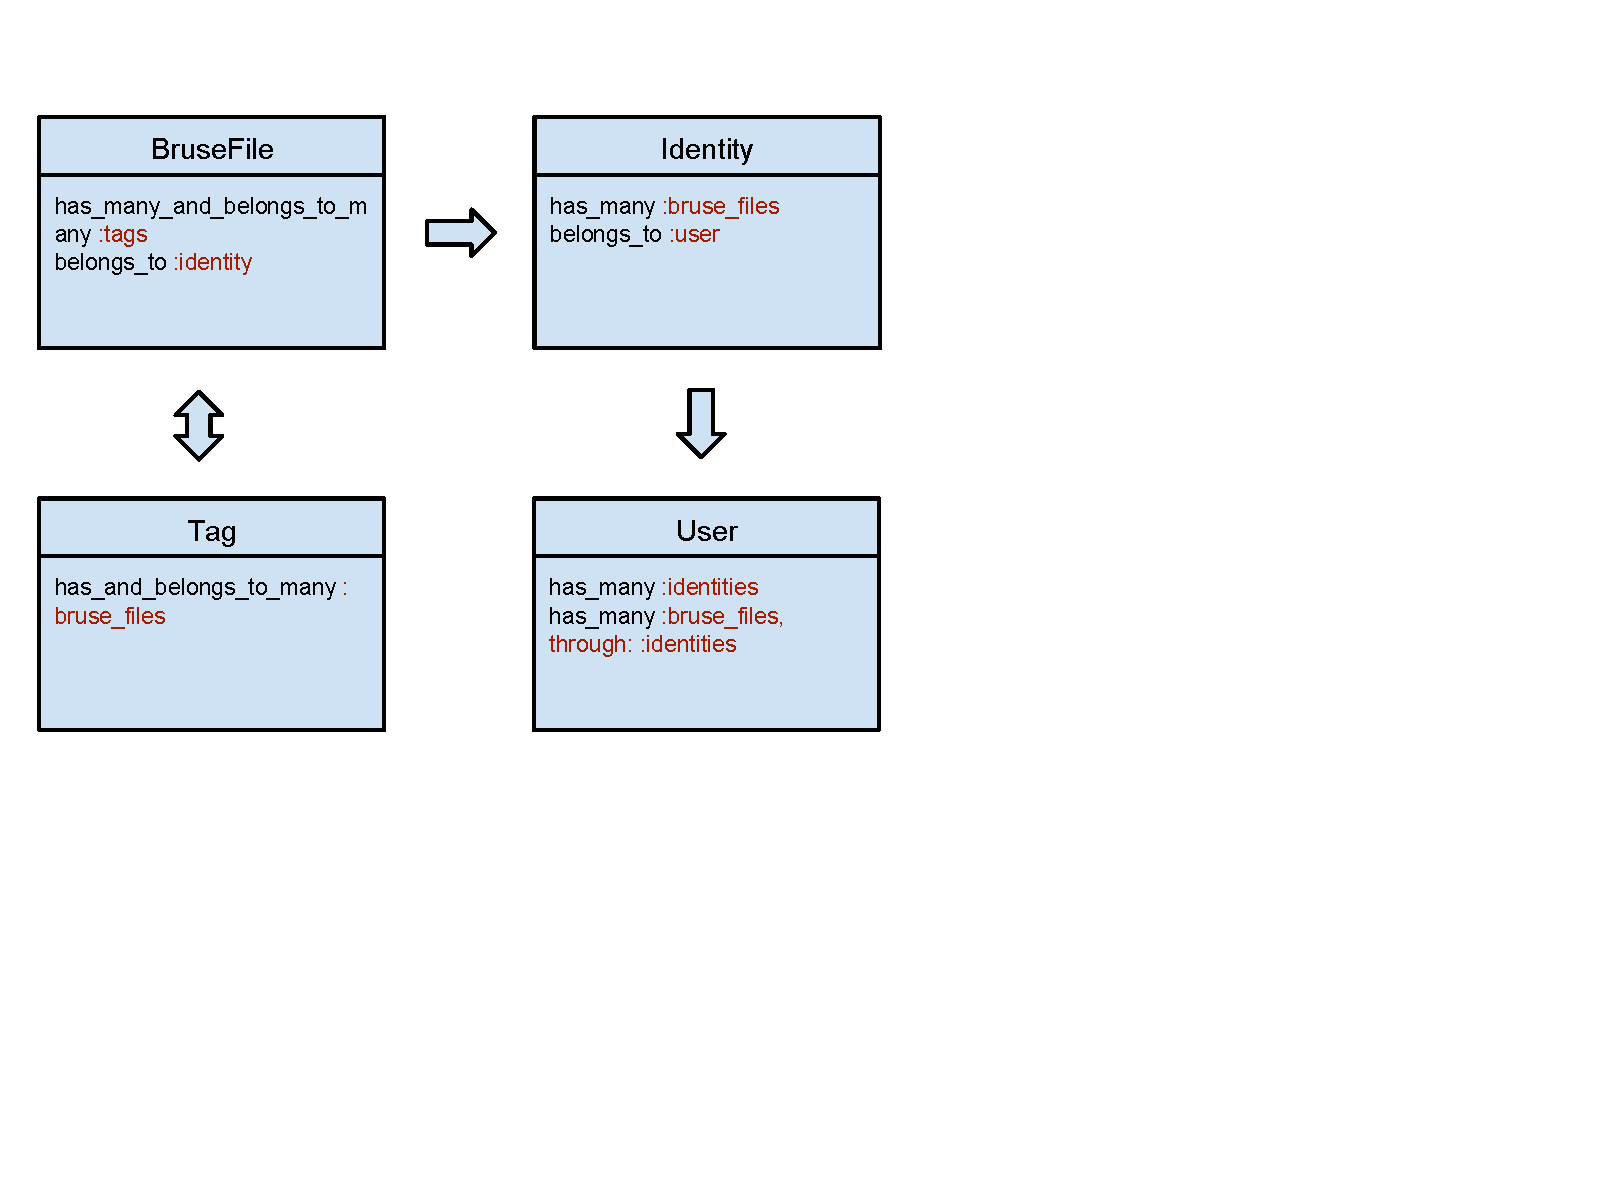
\includegraphics[width=0.7\linewidth]{figures/model.pdf}
    % caption! change the label ref to what you want
    \captionof{figure}{\emph{Systemets \emph{models} och dess relationer.}\label{fig:models}}
\end{Figure}

\texttt{Identity} är en av  systemets viktigaste models. En \texttt{Identity}
är en av tredjepartstjänsterna Google Drive eller Dropbox. Men även den egna
filhanteringen hanteras som en \texttt{Identity} för att hålla det konsekvent
och modulärt. Modellen är viktig för att kunna skilja på vilken
tredjepartstjänst filen tillhör och kunna hantera den därefter.

För att kunna presentera en fil och dess taggar äger \texttt{BruseFile} flera
taggar, men för att även kunna lista filer beroende på en tagg äger varje tagg
flera \texttt{BruseFiles}. Rails löser relationen mellan dessa två genom att
skapa en tabell som heter \texttt{bruse\_files\_tags} enligt figur
\ref{fig:filestags}.

\begin{Figure}
  % center it!
  \centering
    % adjust width as you like, include image from optional folder
    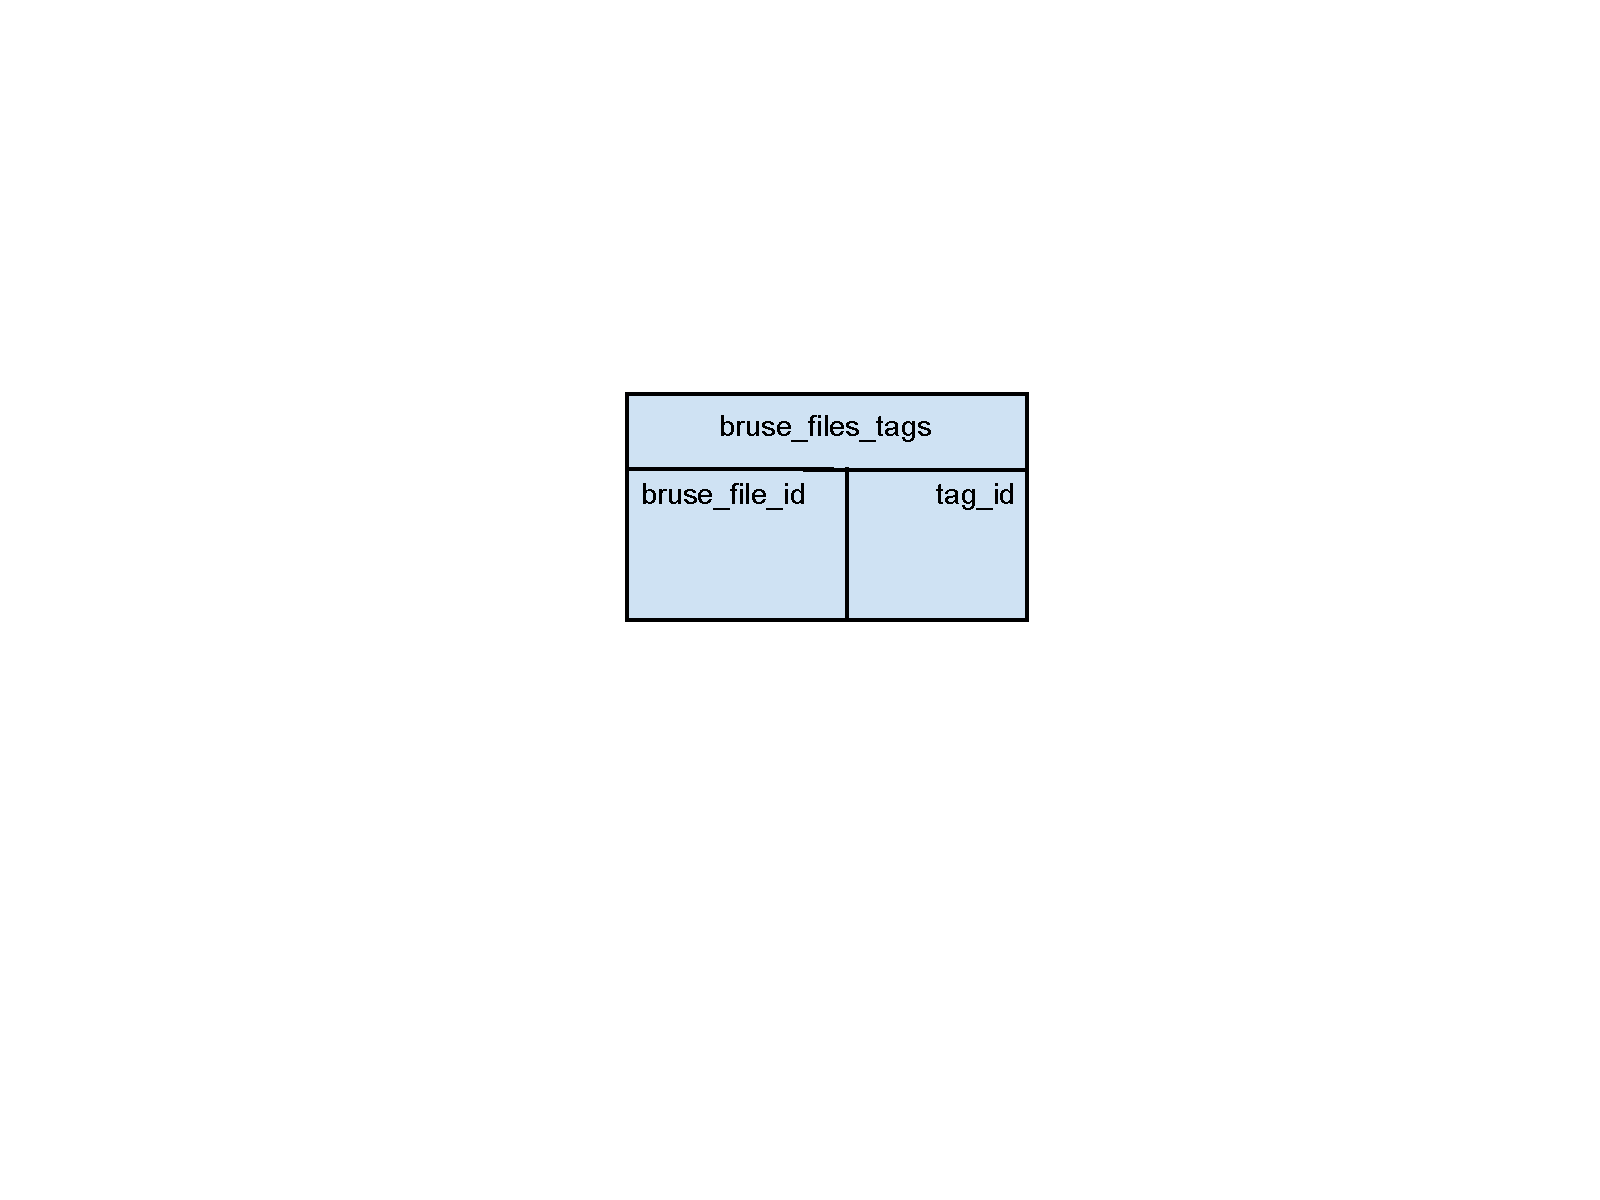
\includegraphics[width=0.3\linewidth]{figures/filestags.pdf}
    % caption! change the label ref to what you want
    \captionof{figure}{\emph{Relation mellan \texttt{BruseFiles} och \texttt{Tags}.}\label{fig:filestags}}
\end{Figure}

Den \emph{controller} som hanterade \texttt{BruseFiles} delades först upp i tre
delar efter en första refaktorering för att sedan bli sex vid utökad
funktionalitet och ytterligare refaktorering. Detta för att filhanteringen
behandlar olika aspekter och behöver då delas upp för att skapa en tydlig
översikt. I figur \ref{fig:filescontroller} beskrivs de olika \emph{controllers}
som används för \texttt{BruseFiles}.

\begin{Figure}
  % center it!
  \centering
    % adjust width as you like, include image from optional folder
    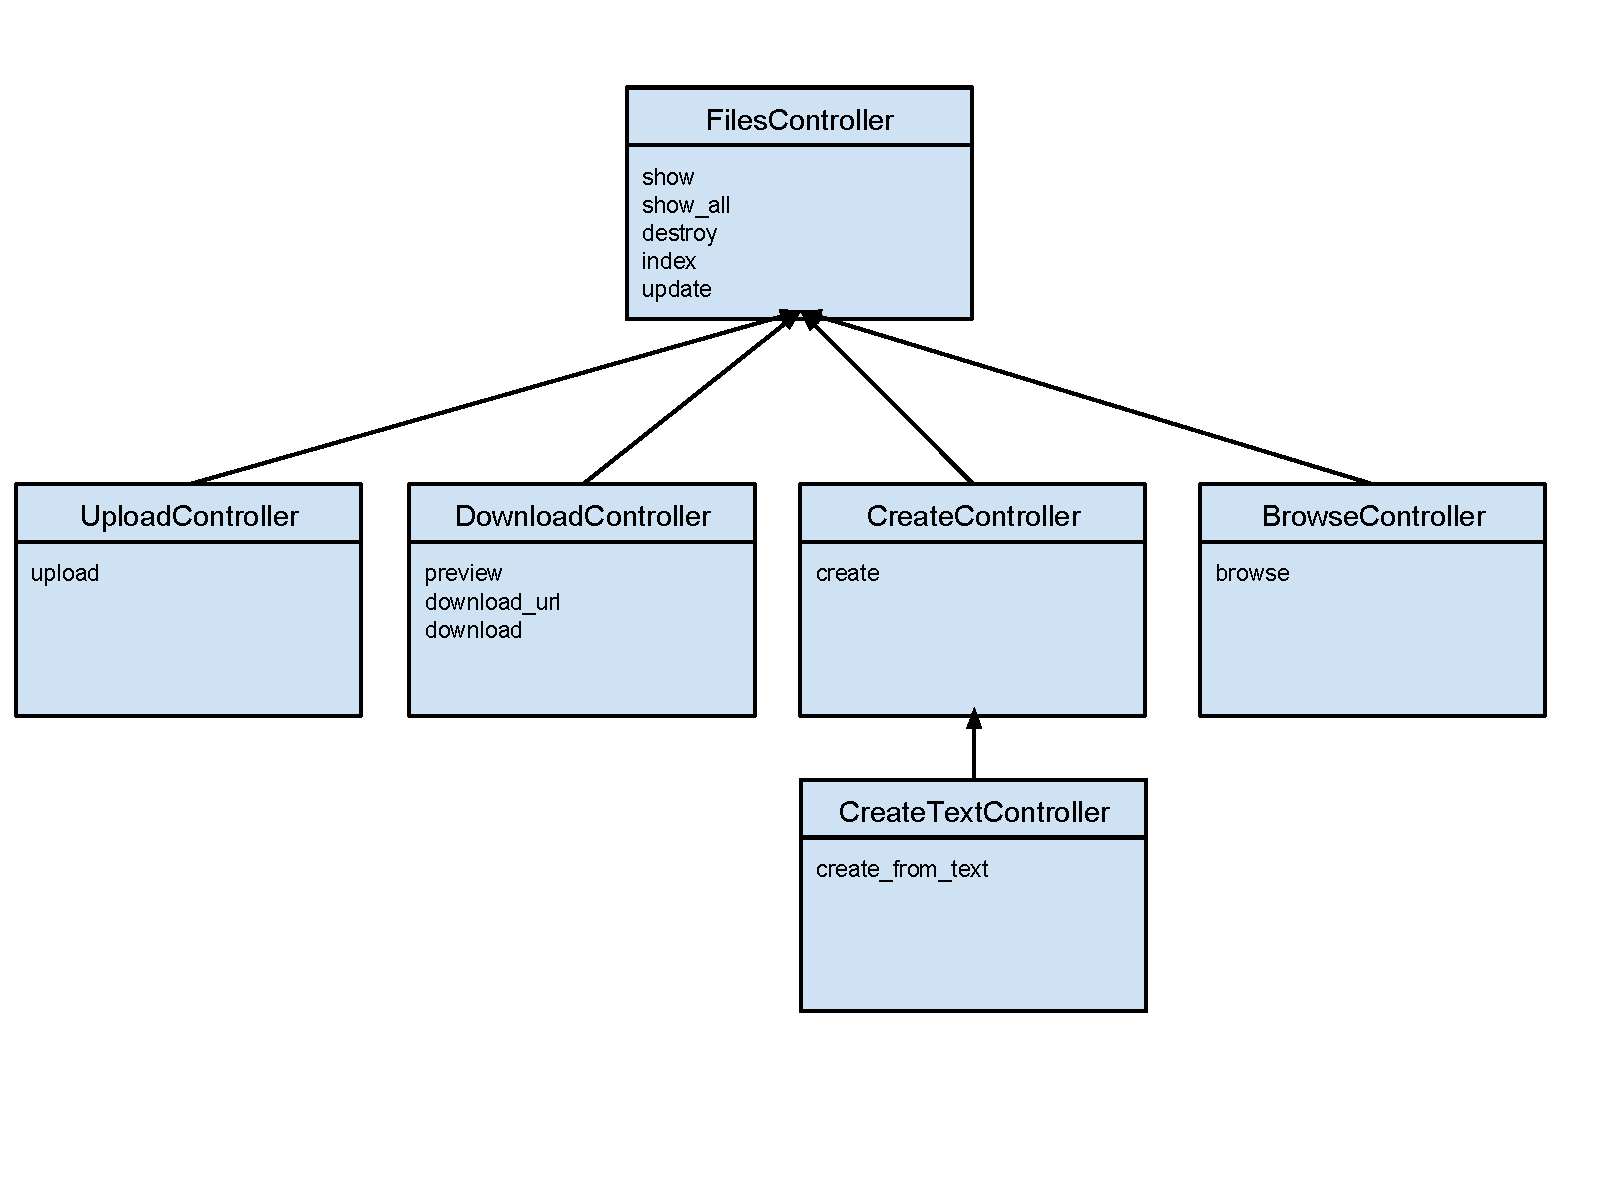
\includegraphics[width=0.9\linewidth]{figures/filescontroller.pdf}
    % caption! change the label ref to what you want
    \captionof{figure}{\emph{Struktur för filrelaterade \emph{controllers}.}\label{fig:filescontroller}}
\end{Figure}

\subsubsection{\texttt{FilesController}}

Denna \emph{controller} är den som alla ärver av, som kan ses i figur
\ref{fig:filescontroller}. Den hanterar de vanligaste metoderna för en fil, de
som handlar om att hitta eller redigera den information om filer som redan är
sparad i databasen. Skillnaden mellan funktionerna \emph{index} och \emph{
show\_all} är att \emph{index} visar alla filer för en identity vid import
medans \emph{show\_all} visar alla filer för alla användarens identities.

\subsubsection{\texttt{BrowseController}}

Hanterar inläsning av mappar från en extern tjänst.

\subsubsection{\texttt{CreateController}}

Skapar ett nytt inlägg i databasen från den information som fås av klienten.
Här finns även validering så att endast tillåtna variabler skickas vidare till
att sparas i databasen. Valideringen av vilken typ variablerna är sker senare i
systemets \emph{model} \texttt{BruseFile}.

\subsubsection{\texttt{CreateTextController}}

Ärver av \texttt{CreateController}. Denna \emph{controller} skapades då
\texttt{create\_text} kräver många fler hjälpfunktioner och valet gjordes att
dela upp dem för att hålla det strukturerat. Många av de funktionerna handlar
om att hantera textsträngen om den är en URL.

\subsubsection{\texttt{DownloadController}}

För att ladda ner filer på ett säkert sätt som kräver att rätt användare är
inloggad skapades en \emph{controller} för att säkerställa detta med ett antal
funktioner. Funktionen \texttt{preview} fick även vara i denna då den hanterar
filer på ett liknande sätt som \texttt{download} gör. \texttt{download\_url}
skapades för att eventuellt implementera en delningsfunktion där flera
användare skulle kunna få tillgång till filen.

\subsubsection{\texttt{UploadController}}

Hanterar filer som ska laddas upp till de olika tjänsterna. Om filen laddas upp
via drag och släpp-metoden eller via ett vanligt formulär tas filerna emot i
olika format. Via drag och släpp-metoden fås filen kodad i \emph{base64}
vilket måste göras om till en så kallad \texttt{Tempfile} och sedan till ett
objekt som är samma som det som fås via formulärsuppladdning \cite{base64}.

\subsection{Klient – Angularjs}

Tillsammans bildar filerna olika komponenter som används för att hantera sina områden, se figur \ref{fig:angularstructure}. De områden som styrs utav Angularjs är

\begin{itemize}
  \item lägga till filer
  \item lägga till taggar till nyligen tillagda filer
  \item söka efter filer
  \item skapa filer från text
  \item drag och släpp-uppladdning
  \item lista filer.
\end{itemize}

\begin{Figure}
  % center it!
  \centering
    % adjust width as you like, include image from optional folder
    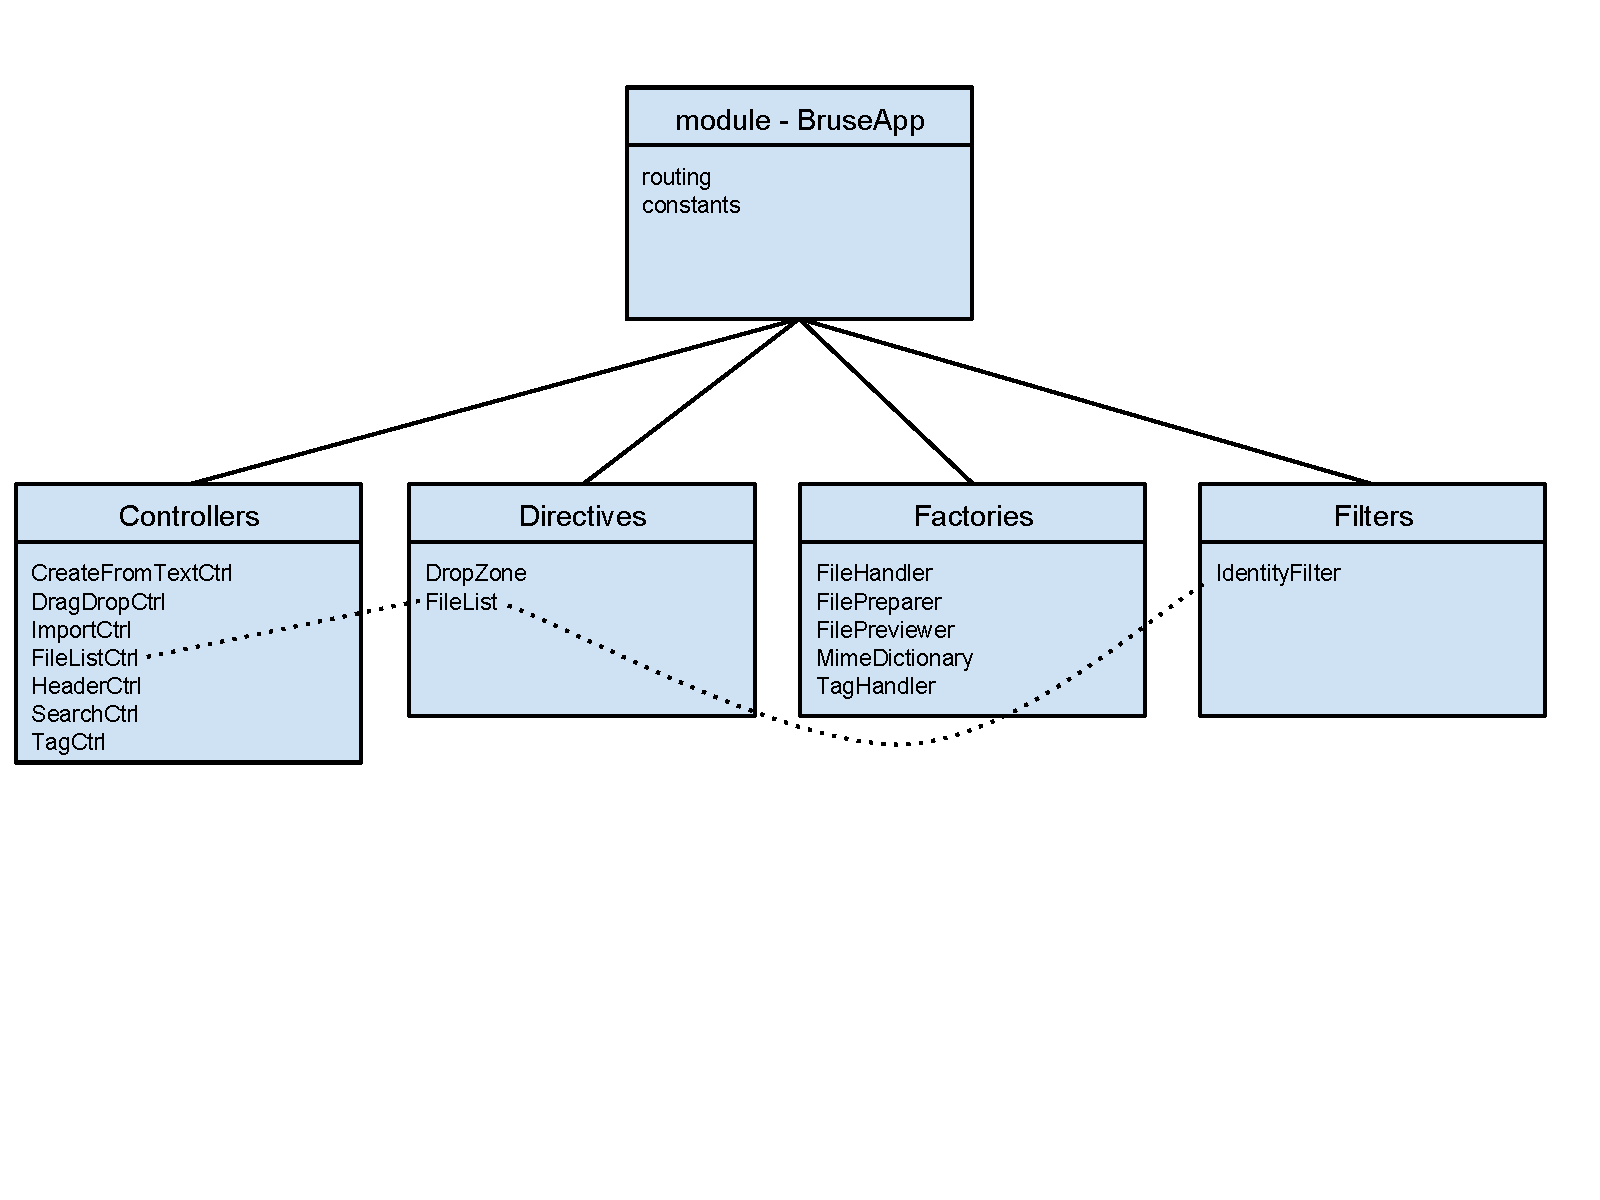
\includegraphics[width=0.9\linewidth]{figures/angularstructure.pdf}
    % caption! change the label ref to what you want
    \captionof{figure}{\emph{Struktur för Angularjs-komponenter.}\label{fig:angularstructure}}
\end{Figure}

Vid import av filer sparas alla de valda filerna i en \emph{array} i
Javascript, sedan när användaren väljer att spara filerna skickas en förfrågan
till serven per fil för att lägga till dem i databasen. Denna \emph{array}
sparas i en global variabel som Angularjs tillhandahåller. Användaren
omdirigeras genom att systemet byter HTML-\emph{template} och URL för att ge
intrycket av att användaren kommer till en ny sida. Men då det är samma session
och ingen ny förfrågan mot serven har gjorts av webbläsaren kan denna nya sida
komma åt samma globala variabel och på så sätt använda sig av de nyligen
tillagda filerna.

Denna lösning använder sig av ett verktyg för Angularjs som heter Angular
Router. Detta verktyg kan hantera olika URL-förfrågor i Javascript och
presentera \emph{templates} och \emph{controllers} som utvecklare specificerat.
Men då en förfrågan av en webbläsare sker först till serven måste även Angular
Router-systemet där vidarebefodra vissa förfrågor till en speciell URL så att
Javascript och Angular Router kan ta över istället för servern.

Angularjs \emph{factories} användes för att: uppdatera och skapa filer, för att visa
filer, för att uppdatera taggar, för att förbereda filer för visning samt för
att hantera olika filtyper. Detta kan exempelvis innebära att
\texttt{MimeDictionary.prettyType()} användes för att skriva ut en fils MIME-
typ (\emph{Multipurpose Internet Mail Extensions}) i ett mer läsbart format
\cite{mime}. Exempelvis ``excel spreadsheet'' istället för
``application/vnd.ms-excel'' och ``c++ file'' istället för ``text/x-c''.

\emph{Factories} användes även för att hantera asynkrona anrop mot servern.
Detta gjorde att utvecklaren kunde veta när anropen var färdiga, till exempel
när en fil hade uppdaterats och vad resultatet blev.

\subsection{Sökning}

För att låta en användare söka efter filer i systemet på ett enkelt och
effektivt sätt delades denna funktion upp så att både servern och klienten
användes för att hantera användarens önskemål. Hos klienten skrev användaren in
sin söksträng som en kombination av ord, ord föregångna av ett nummertecken
``\#'' och ord föregågna av en punkt ``.''. Denna söksträng delades upp efter
respektive typ av ord, och skickades till servern. Servern tog då hand om denna
samling som generella ord att söka efter, taggar att söka efter samt filtyper
att söka efter. Då en användare skrev söktermen ``hej \#hälsning .txt'' sökte
alltså servern efter filer och taggar som innehöll ordet ``hej'' i sitt namn,
hade taggen hälsning och var en textfil. Resultatet presenterades sedan för
användaren utav klienten.

\section{Tredjepartsmjukvara}

Devise är ett tillägg till Ruby on Rails som ger ett paket för
användarhantering, färdigt att användas. Då beslutet om att användare även
skulle kunna logga in med e-postadress och lösenord insågs det samtidigt att en
tredjepartsmjukvara skulle vara nödvändigt för att hålla tidsramen. Devise
valdes för att det gav den mest kompletta lösningen med färdiga \emph{views},
modifierbara \emph{controllers} och enkel \emph{model}-påbyggnad. Devise har
också inbyggda funktioner som tillsammans med Rails e-postssystem skickar e-
post till användare då de till exempel registrerar sig eller behöver hjälp med
att återställa sitt lösenord.

Carrierwave ger utvecklarna verktyg för att hantera uppladdningen av filer.
Genom att endast specificera inställningar för var filen ska sparas och så
vidare fås en modul som kan användas i de \emph{controller}-metoder som behövs.

Fuzzily skapar för varje ny instans av specificerade models så kallade
\emph{trigrams} över valda kolumner. \emph{Trigrams} delar upp ett ord och
grupperar det om tre tecken i taget \cite{n-grams}. För varje ny gruppering
förflyttas den ett steg vilket gör att det skapas flera olika kombinationer.
För ett ord skulle det resultera i flera olika bokstavskombinationer av
grundordet. Exempelvis skulle ordet ``bruse'' med hjälp av trigrams bli
\texttt{[b, br, bru, rus, use, se, e]}. Under implementationen av Fuzzily
upptäcktes det att  numeriska eller nordiska tecken inte sparades i trigrams.
Tack vare att Fuzzily är skrivet i öppen källkod kunde problemet åtgärdas genom
att ändra koden.

Delayed Job användes för att kunna skjuta upp skapandet av \emph{trigrams}.
Genom att spara kommande jobb i en lista kunde skapandet ske utan att blockera
en förfrågan från användaren. Istället skedde detta i en ny process i
bakgrunden.

Jstag är ett tillägg till Angularjs som konverterar användarens inskrivning
utav taggar till visuella objekt för att tydliggöra för användaren hur dess
inskrivning tolkas utav systemet. Även detta tillägg hade brister då olika
objekt kopierades utav systemet utan att samtliga tvåvägsbindningar behölls som
kunde åtgärdas tack vare att det var skrivet med öppen källkod.

Magnific Popup gör att filerna som laddas upp till systemet går att
förhandsgranska i samma vy som användaren befinner sig på. För att en viss
filtyp ska kunna förhandsgranskas krävs det att man lägger till en definition
för filtypen i hjälpfunktionen \texttt{MimeDictonary}. Magnific Popup använder
samma teknik som webbläsaren gör för att förhandsgranska en fil vilket gör att
filtyper som bilder, filmer, musik och textfiler går att öppna.

\subsection{Filhantering}

Då en fil lagrades i systemet var det två attribut som var centrala. Dels
varifrån filen sparats – om den importerades från en extern tjänst som Google
Drive eller Dropbox, eller om den lagrades i systemets lokala fillagring. Dels
också en textsträng som motsvarar hur den aktuella tjänsten som filen tillhör
separerar filen från övriga filer . Denna textsträng kallas i systemet för
\texttt{foreign\_ref}. För Google Drive är detta en slumpmässig bokstavs- och
sifferkombination, för Dropbox är detta sökvägen till filen. För den lokala
filhanteringen är detta namnet på filen efter att den sparats på servern, också
detta en slumpad bokstavs- och sifferkombination.

\subsection{Gränssnitt}

Systemet utvecklades för att ge användaren en enkel och tillgänglig upplevelse
med ljusa färger och tydliga uppdelningar mellan systemets komponenter. Nedan
visas skärmdumpar från systemets olika delar. I figur \ref{fig:dump1} till
\ref{fig:dump5} visas skärmdumpar från systemet.

\begin{Figure}
  % center it!
  \centering
    % adjust width as you like, include image from optional folder
    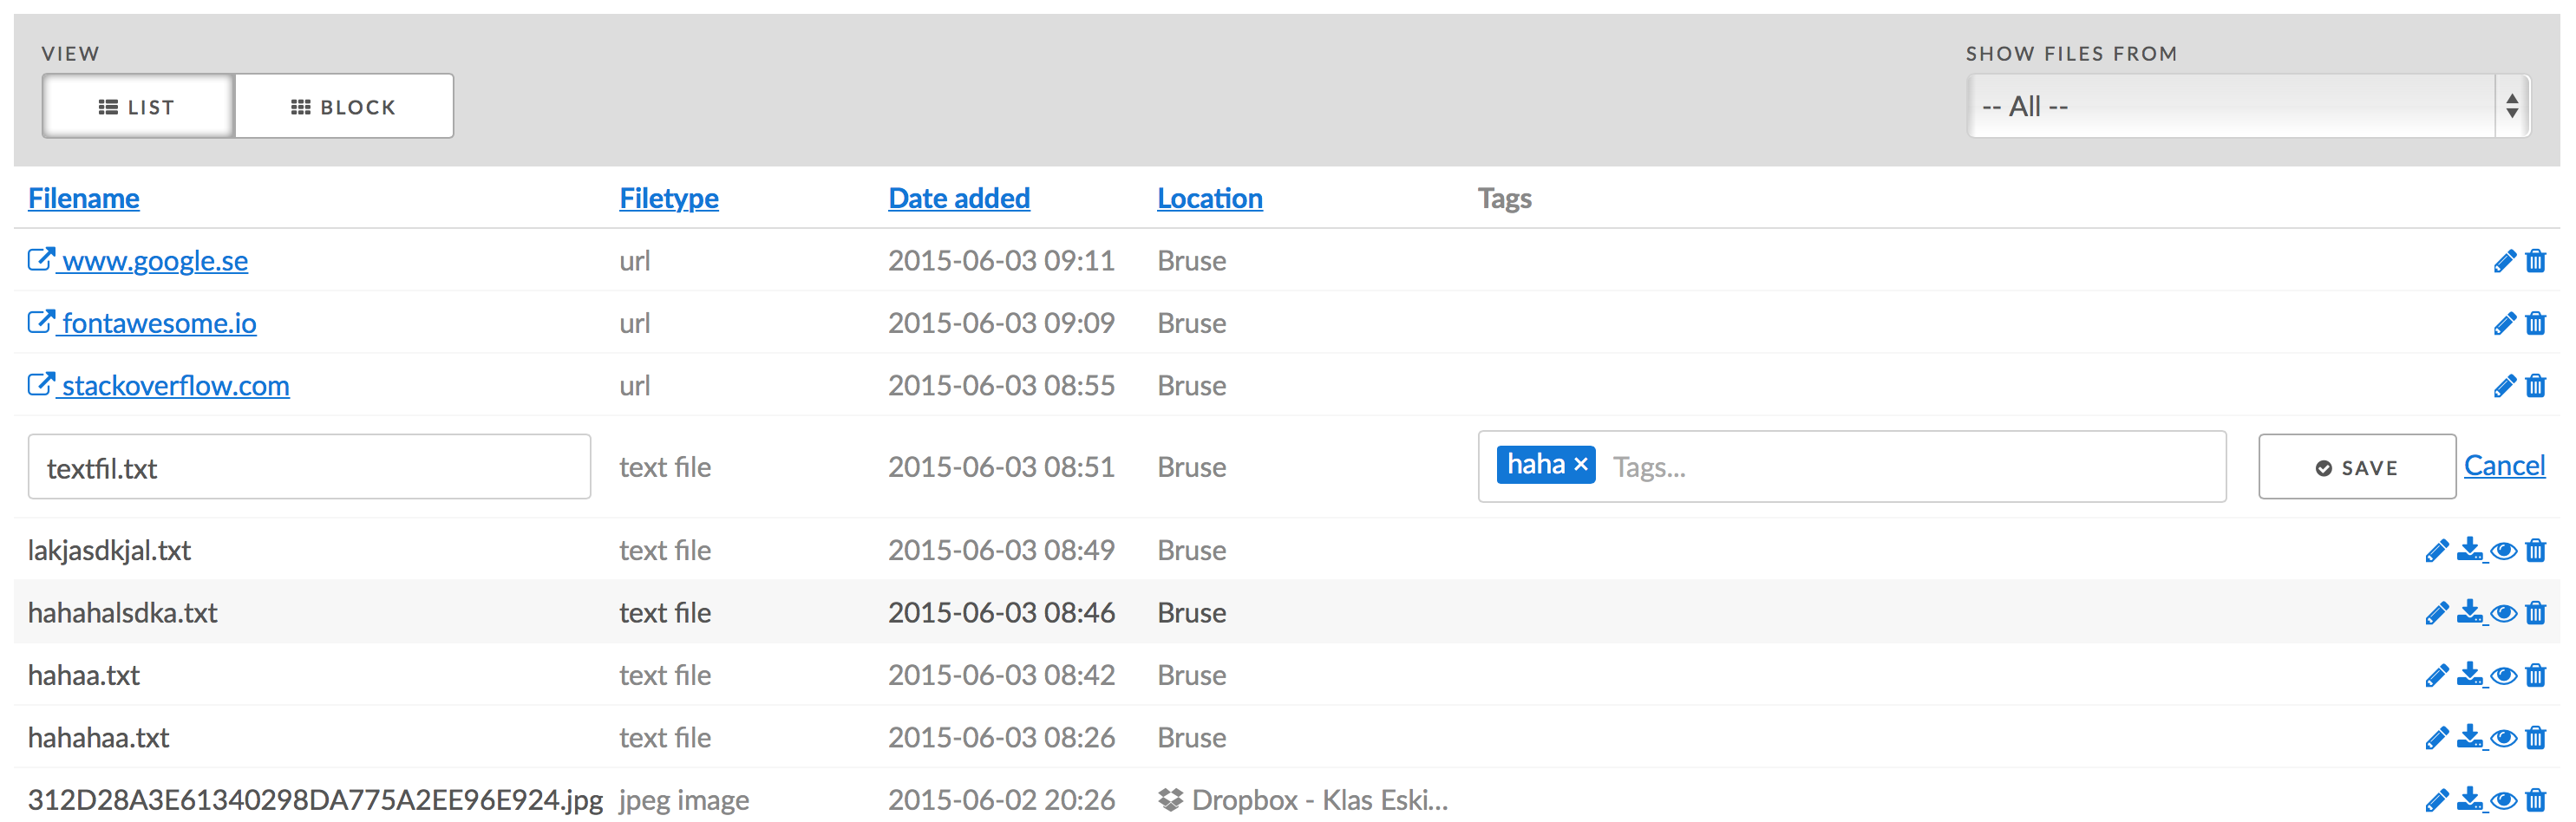
\includegraphics[width=0.9\linewidth]{figures/screenshots/dump1.png}
    % caption! change the label ref to what you want
    \captionof{figure}{\emph{Systemets lista över dess filer. En fil redigeras.}\label{fig:dump1}}
\end{Figure}

\begin{Figure}
  % center it!
  \centering
    % adjust width as you like, include image from optional folder
    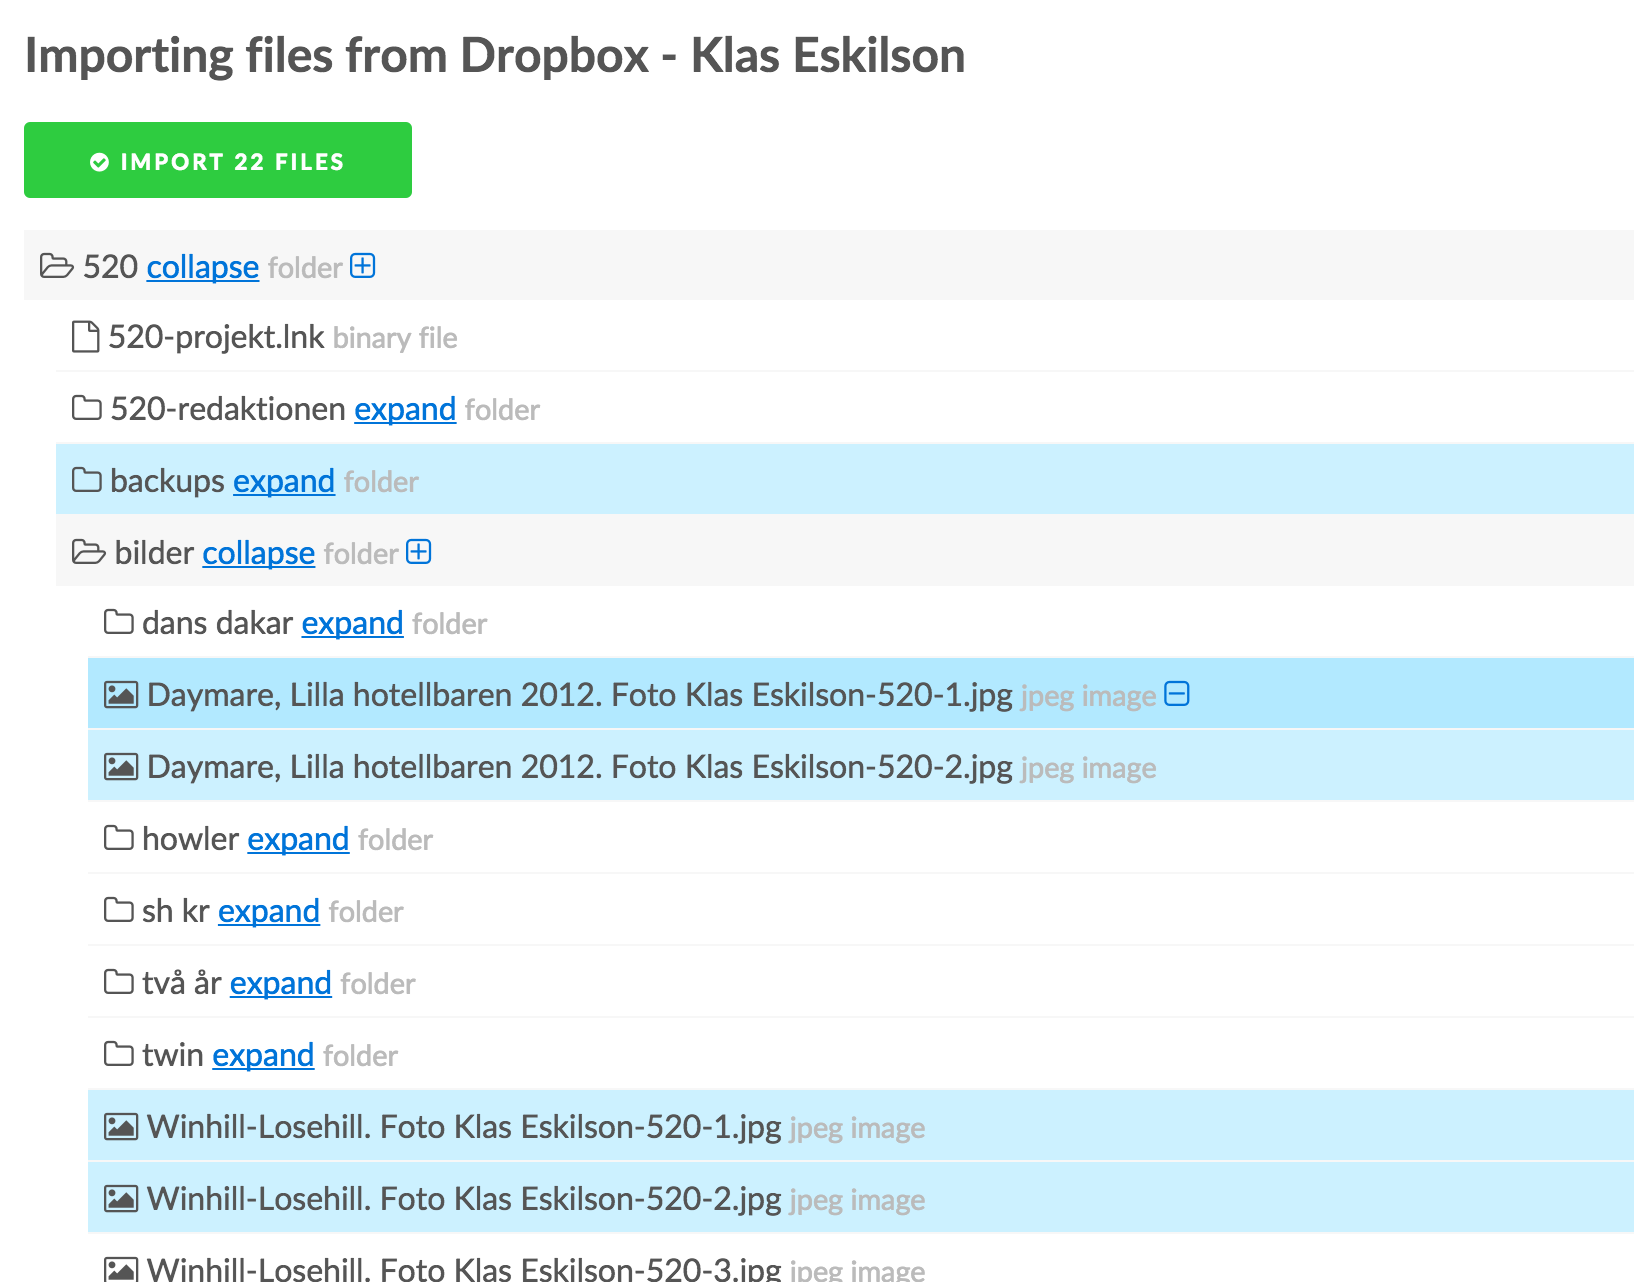
\includegraphics[width=0.8\linewidth]{figures/screenshots/dump2.png}
    % caption! change the label ref to what you want
    \captionof{figure}{\emph{Filimport.}\label{fig:dump2}}
\end{Figure}

\begin{Figure}
  % center it!
  \centering
    % adjust width as you like, include image from optional folder
    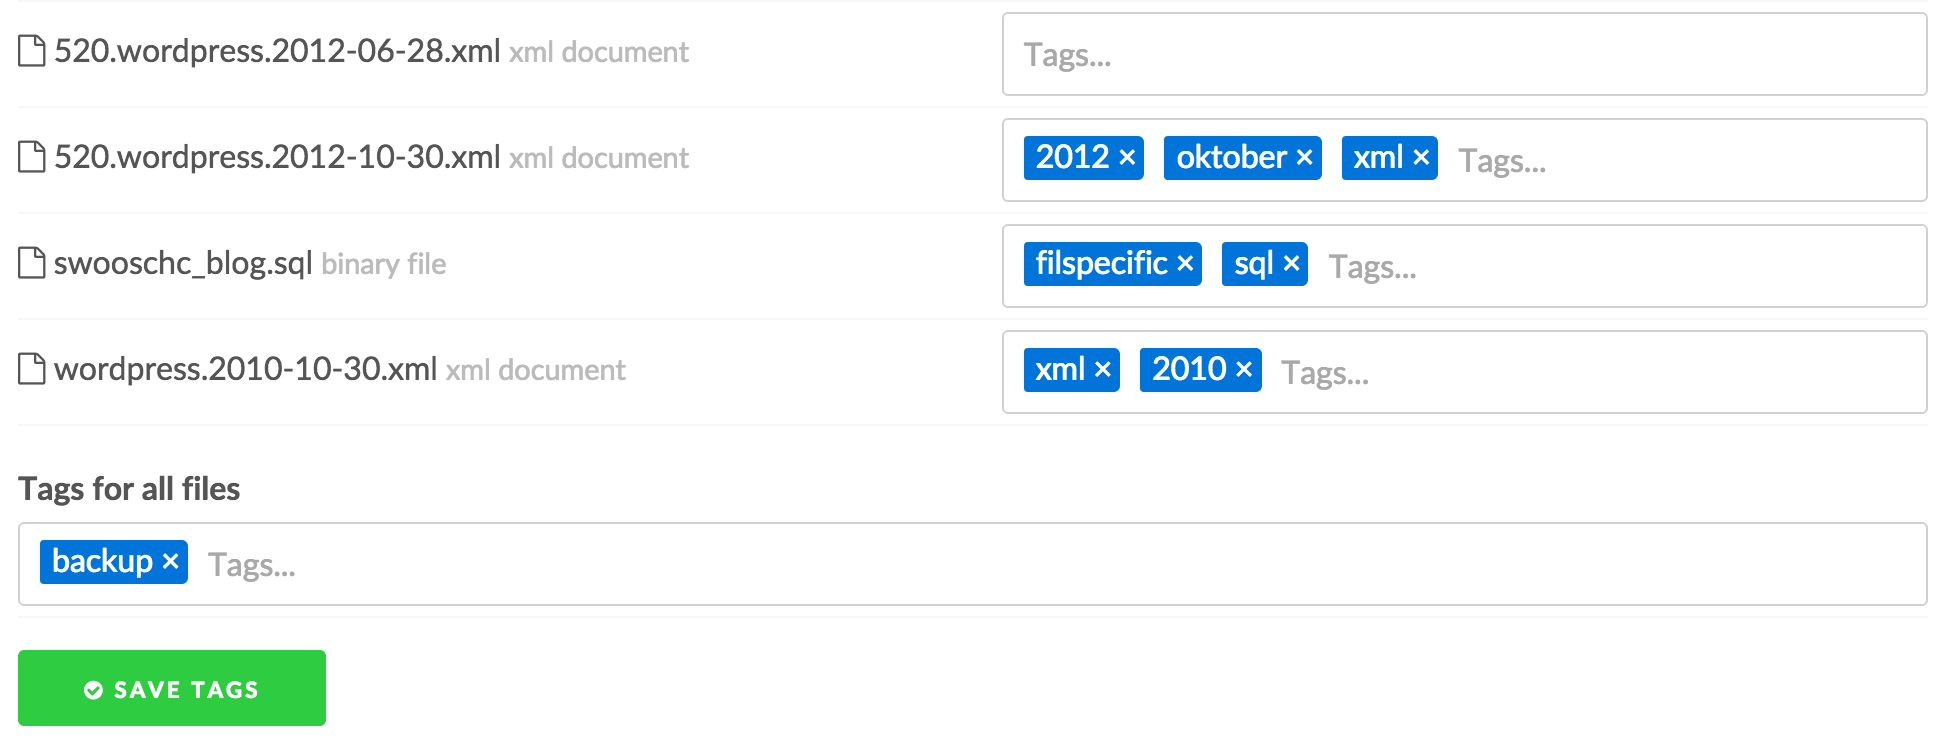
\includegraphics[width=0.7\linewidth]{figures/screenshots/dump3.png}
    % caption! change the label ref to what you want
    \captionof{figure}{\emph{Taggning av filer efter import.}\label{fig:dump3}}
\end{Figure}

\begin{Figure}
  % center it!
  \centering
    % adjust width as you like, include image from optional folder
    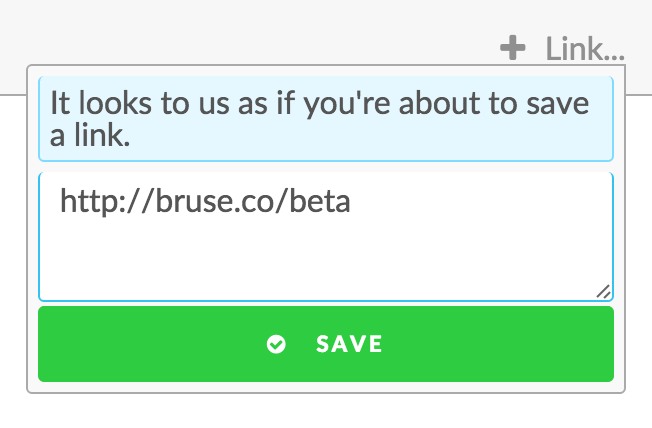
\includegraphics[width=0.4\linewidth]{figures/screenshots/dump4.png}
    % caption! change the label ref to what you want
    \captionof{figure}{\emph{Sparande av bokmärke via textfält.}\label{fig:dump4}}
\end{Figure}

\begin{Figure}
  % center it!
  \centering
    % adjust width as you like, include image from optional folder
    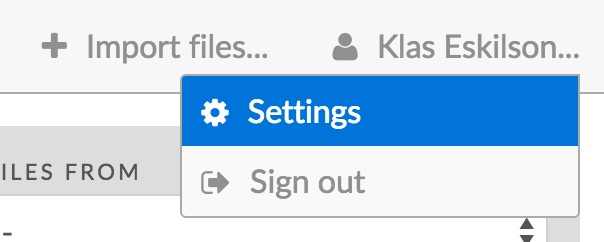
\includegraphics[width=0.4\linewidth]{figures/screenshots/dump5.png}
    % caption! change the label ref to what you want
    \captionof{figure}{\emph{Öppen undermeny.}\label{fig:dump5}}
\end{Figure}

\section{Utvecklingsmetodik}

Arbetet följde Scrum som utvecklingsmetodik vilket har resulterat i en tydlig
och strukturerad arbetsgång. Korta scrummöten i början av varje arbetsdag har
förhindrat onödigt arbete samt att alla utvecklare är insatta i arbetet. Varje
sprintgranskning och sprintåterblick har givit en tydlig bild om vad som gjorts
och behöver göras för att nå nästa förbättring av produkten.

\section{Versionshantering och kodgranskning}

Användningen av Github gjorde att det alltid fanns en fungerande programversion
i \emph{develop}-förgreningen. Systemet växte i funktionalitet allt eftersom
nya tillägg från \emph{pull requests} godkändes. Om det inte fanns behov av
kodning fanns det alltid behov av att granska \emph{pull requests}. Antal
\emph{pull requests} och \emph{commits} varierade från person till person.
\emph{Commits} från varje gruppmedlem och övrig statistik finns i bilaga [].
